\chapter{Zusammenfassender Bericht}
\label{sec.zusammenfassender_bericht}
Das zwölfwöchige Pflichtpraktikum wurde in der Abteilung ADAS Driving Functions/ Chauffeur Functions der Firma Continental Teves AG \& Co. oHG in Eschborn absolviert. Im Folgenden wird zu Beginn eine Übersicht der Tätigkeitsfelder der Abteilung, in welcher das Praktikum unter Bearbeitung interdisziplinärer Tätigkeitsfelder absolviert wurde, gegeben, bevor darauf folgend die Aufgaben und Tätigkeiten, welche während des Praktikums bearbeitet wurden, beschrieben werden. 

Die Abteilung ist im Bereich des automatisierten Fahrens tätig. Das automatisierte Fahren lässt sich hierbei nach SAE-Standard J3016 in insgesamt fünf Automatisierungsgrade unterteilen. Beschreibt der Automatisierungsgrad des Levels 0 einen Zustand, in dem der Fahrer selbst fährt und im Zuge dessen alle Manöver wie Beschleinigung oder Bremsung selbst durchführt, so handelt es sich bei dem Automatisierungsgrad des Level 5 um einen komplett autonomen Zustand, in welchem der Fahrer keinerlei Beitrag zum Kontrollieren des Fahrzeugs leistet, außer die Vorgabe des Fahrziels sowie des Starten des Systems [Quelle: xxx]. Die Abteilung, in welcher das Pflichtpraktikum absolviert wurde, ist in diesem Kontext innerhalb des Automatisierungsgrades Level 2+ anzusiedeln. Funktionen wie automatisches Einparken, Spurhalten, Abbremsen auf andere Verkehrsteilnehmer sind hier im Fahrzeug integriert. Ebenso sind Fahrfunktionen wie ACC (Adaptive Cruise Control), welches einen konstanten Abstand zu vor dem eigenen Fahrzeug befindlichen Verkehrsteilnehmern in Abhängigkeit ihrer Geschwindigkeiten einhält. Ein besonderer Arbeitsschwerpunkt der Abteilung liegt auf dem automatisierten Spurwechsel, welcher laut SAE-Standard J3016 formell im Automatisierungsgrad Level 3 anzuordnen ist.

Praktikumstätigkeiten
Der erste Einsatzbereich fand im Bereich des automatisierten Spurwechsels im High-Way-Kontext, also auf der Autobahn, statt. Im Folgenden wird die ebenfalls in der Abteilung verwendete Fachsprache benutzt, die verwendeten Abkürzungen werden bei der ersten Erwähnung erläutert und finden sich des Weiteren im Abkürzungsverzeichnis dieses Berichtes (siehe Abkürzungsverzeichnis). Das Vehikel, für welches die automatisierten Funktionen implementiert werden sollen, wird als Ego bezeichnet. Andere Verkehrsteilnehmer werden mit TPO (Traffic Participant Object) gekennzeichnet. Eine Fahrspur wird mit dem Begriff Lane betitelt, die die Lane jeweils nach rechts und links begrenzenden Fahrbahnmarkierungen entsprechend mit Lane-Marker. Die Fahrspur, auf dem sich das Ego-Fahrzeug aktuell befindet, wird mit Ego-Lane bezeichnet. Im Kontext eines geplanten Fahrspurwechsels erhält die Fahrspur, die als Ergebnis des Spurwechsels dient, den Namen Target-Lane.

%%%%%% Hier einfügen Diagramm Systemarchitektur
%%%%%% Fragen beantworten, was uns zur Verfügung steht, wir entwickeln den Trajektorienplaner, welcher dann im Folgenden auf verschiedene Szenarien angewandt wird.
Das erste betrachtete Szenario umfasst ein Ego-Fahrzeug, welches sich zum Startzeitpunkt auf der rechten Spur einer zweispurigen Autobahn befindet. Vor dem Ego-Fahrzeug befindet sich auf der rechten Spur ein TPO. Der Set-Speed, also die gewollte Geschwindigkeit, beträgt 100 km/h. Da das TPO auf der Ego-Lane jedoch nur eine Geschwindigkeit von 80 km/h vorweist, fährt das Ego mit aktiviertem ACC mit konstantem Abstand hinter dem TPO her. Auf der Target-Lane befindet sich ebenfalls ein TPO, welches mit konstanten 80 km/h fährt. Der Wunsch eines Fahrspurwechsels wird, wie bereits erwähnt, durch das Setzen des Blinkers in die gewünschte Richtung signalisiert. Darauf folgend wird unter zu Hilfe nahme der Umgebung eine abzufahrende Bahn geplant. Da diese Bahn keine visuellen Informationen bereitstellt, erfolgte eine solche Visualisierung in einem ersten Schritt innerhalb des Praktikums. Mittels der Programmiersprache Python wurde das anfangs beschriebene High-Way-Szenarion simuliert und visualisiert. Ein erstes Konzept der Visualisierung ist in Abbildung xy zu sehen. 

\begin{figure}[!ht]
	\begin{center}
		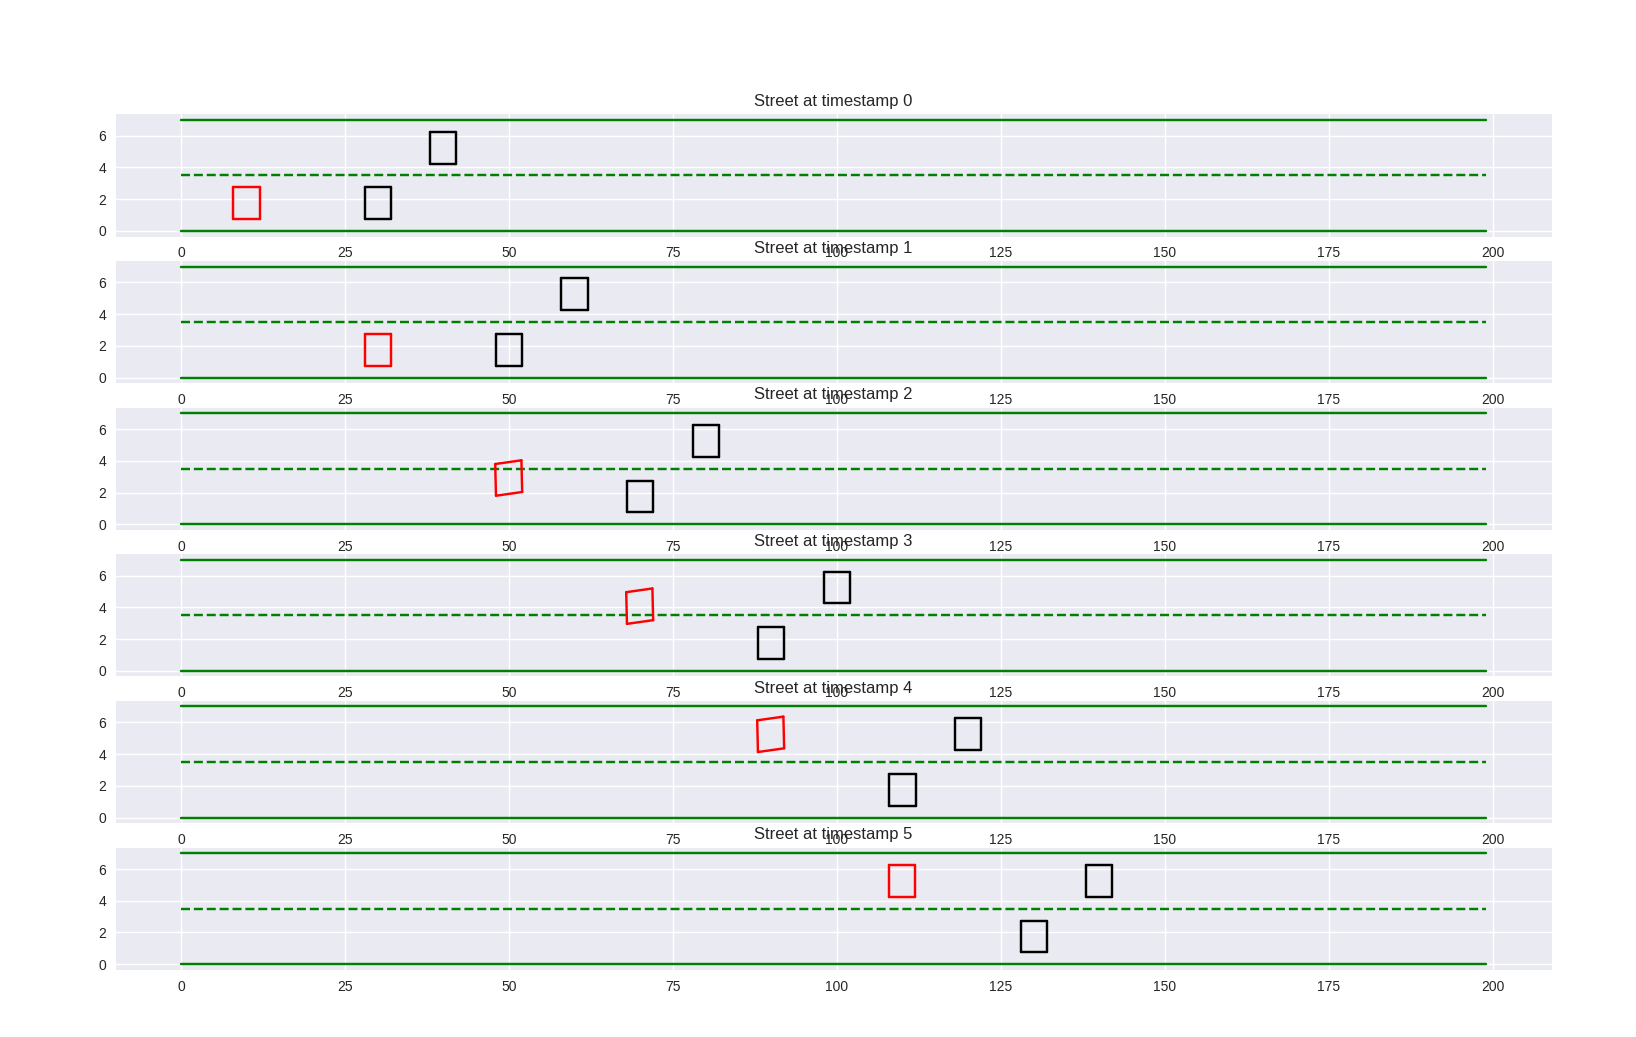
\includegraphics[width=1.0\linewidth]{Abbildungen/bericht/lanechange_visualization}
		\caption{Visualisierung Highway-Spurwechsel in Python}
		\label{fig.highway_spurwechsel_python}
	\end{center}
\end{figure} 

In rot dargestellt sind hier die schemenhaften Umrisse des Ego-Fahrzeuges, in schwarz dargestellt sind die TPO's auf der Ego-Lane sowie auf der Target-Lane. Über mehrere Zeitschritte hinweg ist die Veränderung der Position sowie der Orientierung der Verkehrsteilnehmer während des Spurwechsels aufgetragen. Die Lane-Marker sind im Diagramm in grün eingezeichnet. 
In einem nächsten Schritt erfolgte die Portierung des Visualisierungskonzeptes von der Programmiersprache Python in die Programmiersprache C++. Diese Portierung wurde durch die Tatsache, dass die Planungsalgorithmen für den Spurwechsel ebenfalls in C++ geschrieben sind.

% Kann man hier ggf noch ein Bild von der Gesamtübersicht reinpacken, wie z.B. von dem Eingang der Sensordaten etc? Frank fragen.

Ein weiterer Grund für die Portierung ergibt sich daraus, dass die Datentypen, welche in der urpsprünglichen Python-Visualisierung noch selbst erstellt waren, nun auf die von den tatsächlichen Algorithmen verwendeten Datentypen angepasst werden mussten. Bild xy stellt die fertige Visualisierung dar, der Übersichtlichkeit halber sind nur zehn Zeitschritte des Spurwechsels dargestellt. Im Gegensatz zu Bild xy ist die C++ - Portierung um einige Funktionalitäten ergänzt.

\begin{figure}[!ht]
	\begin{center}
		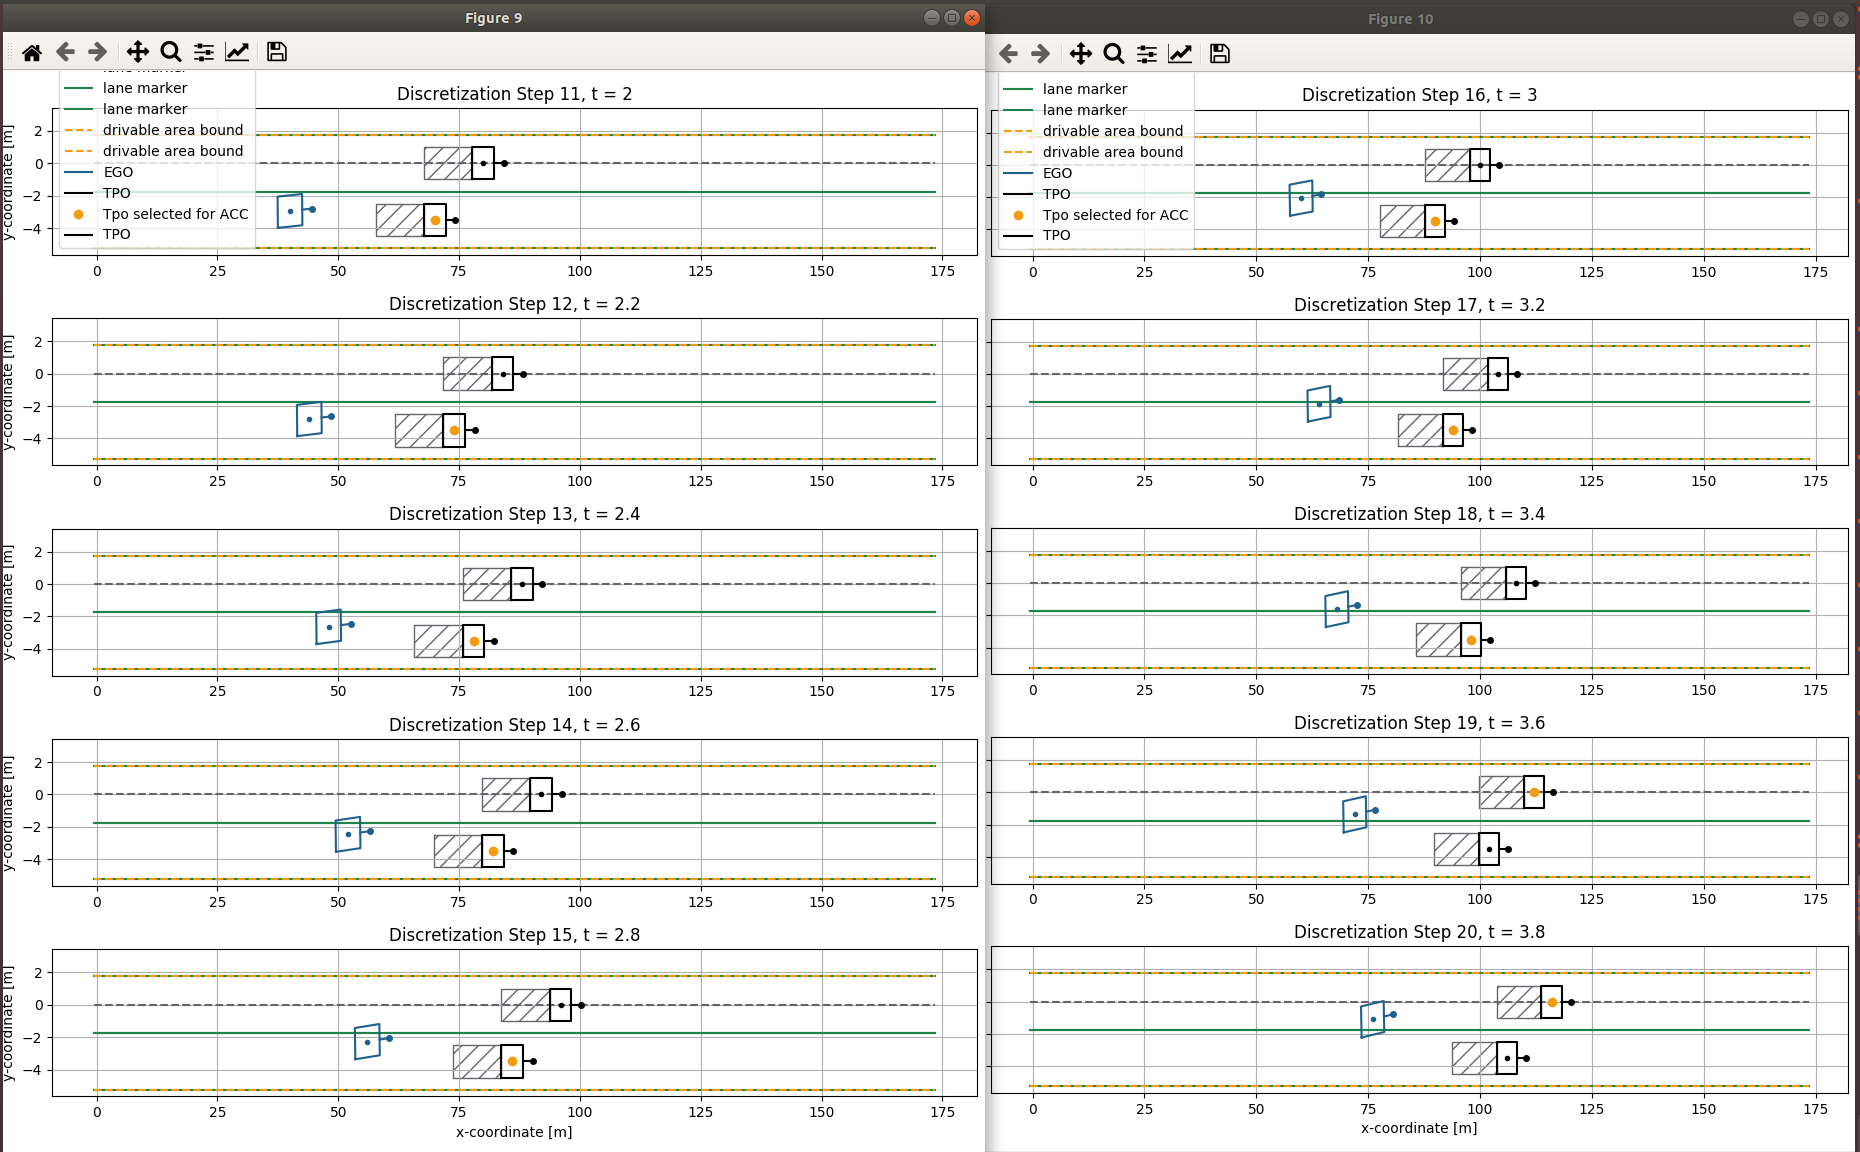
\includegraphics[width=1.0\linewidth]{Abbildungen/bericht/unittest_lc_visu_clion_part1}
		\caption{Visualisierung Highway-Spurwechsel in der C++ -Portierung}
		\label{fig.highway_spurwechsel_clion}
	\end{center}
\end{figure} 

Hinter den beiden TPO's sind so nun Sicherheitszonen eingezeichnet, welche das Ego-Fahrzeug zu keinem Zeitpunkt interferieren darf. Mit einem gelben Punkt gekennzeichnet ist das TPO, auf welches aktuell ACC gefahren wird, d.h. anhand welchen Verkehrsteilnehmers die aktuelle Ego-Geschwindigkeit eingestellt wird, um die grau schraffierte Sicherheitszone nicht zu verletzen (siehe Bild xy). Ab dem Zeitpunkt 19  wird das TPO auf der Target-Lane als ACC-Ziel gewählt (Wechsel des gelben Punktes). Der longitudinale Abstand zu dem TPO auf der vorherigen Lane ist irrelevant, da bereits durch den Spurwechsel ein genügend großer, lateraler Abstand zwischen diesem TPO und dem Ego-Fahrzeug geschaffen wurde. Mit dem Setzen des Blinkers wird ab Zeitschritt 11 mit der grau gestrichelten Linie in den Grafiken die Soll-Linie des Ego-Fahrzeugs eingezeichnet, d.h. die gewünschte Bahn.

% Hier vllt. die Bilder von den Gewichten einfügen. Spurwechsel wird dadurch ausgelöst, dass ein Minimierungsproblem gelöst werden soll.

In einem weiteren Schritt mussten Simulationsdaten verschiedener Spurwechsel-Szenarien gesammelt werden. Hierzu wurde auf die Software \glqq CarMaker\grqq{} der Firma IPG Automotive GmbH zurückgegriffen, welche Simulationen verschiedenster Verkehrssituationen ermöglicht. Mittels der Software wurden insgesamt drei Szenarien eines Spurwechsels erstellt. Bei allen Szenarion besteht die Ausgangssituation aus zwei vor dem Ego-Fahrzeug fahrenden TPO's, jeweils eines auf der Ego-Lane sowie eines auf der Target-Lane. In \glqq Szenario 1\grqq{} bewegt sich das TPO auf der Target-Lane 10 km/h schneller als das TPO auf der Ego-Lane, und behält während des Spurwechsels des Ego-Fahrzeugs seine Geschwindigkeit bei. In \glqq Szenario 2\grqq{} bewegt sich das TPO auf der Target-Lane 10 km/h langsamer als das TPO auf der Ego-Lane und behält ebenfalls seine Geschwindigkeit während des Spurwechsels des Ego-Fahrzeuges bei. \glqq Szenario 3\grqq{} ähnelt \glqq Szenario 1\grqq{} bis auf die Tatsache, dass das TPO auf der Target-Lane während des Spurwechsels seine Geschwindigkeit von 60 km/h auf 40 km/h reduziert. Einen grafischen Überblick der Fahrspurwechsel geben die Abbildungen xx-xx.

\begin{figure}[!ht]
	\begin{center}
		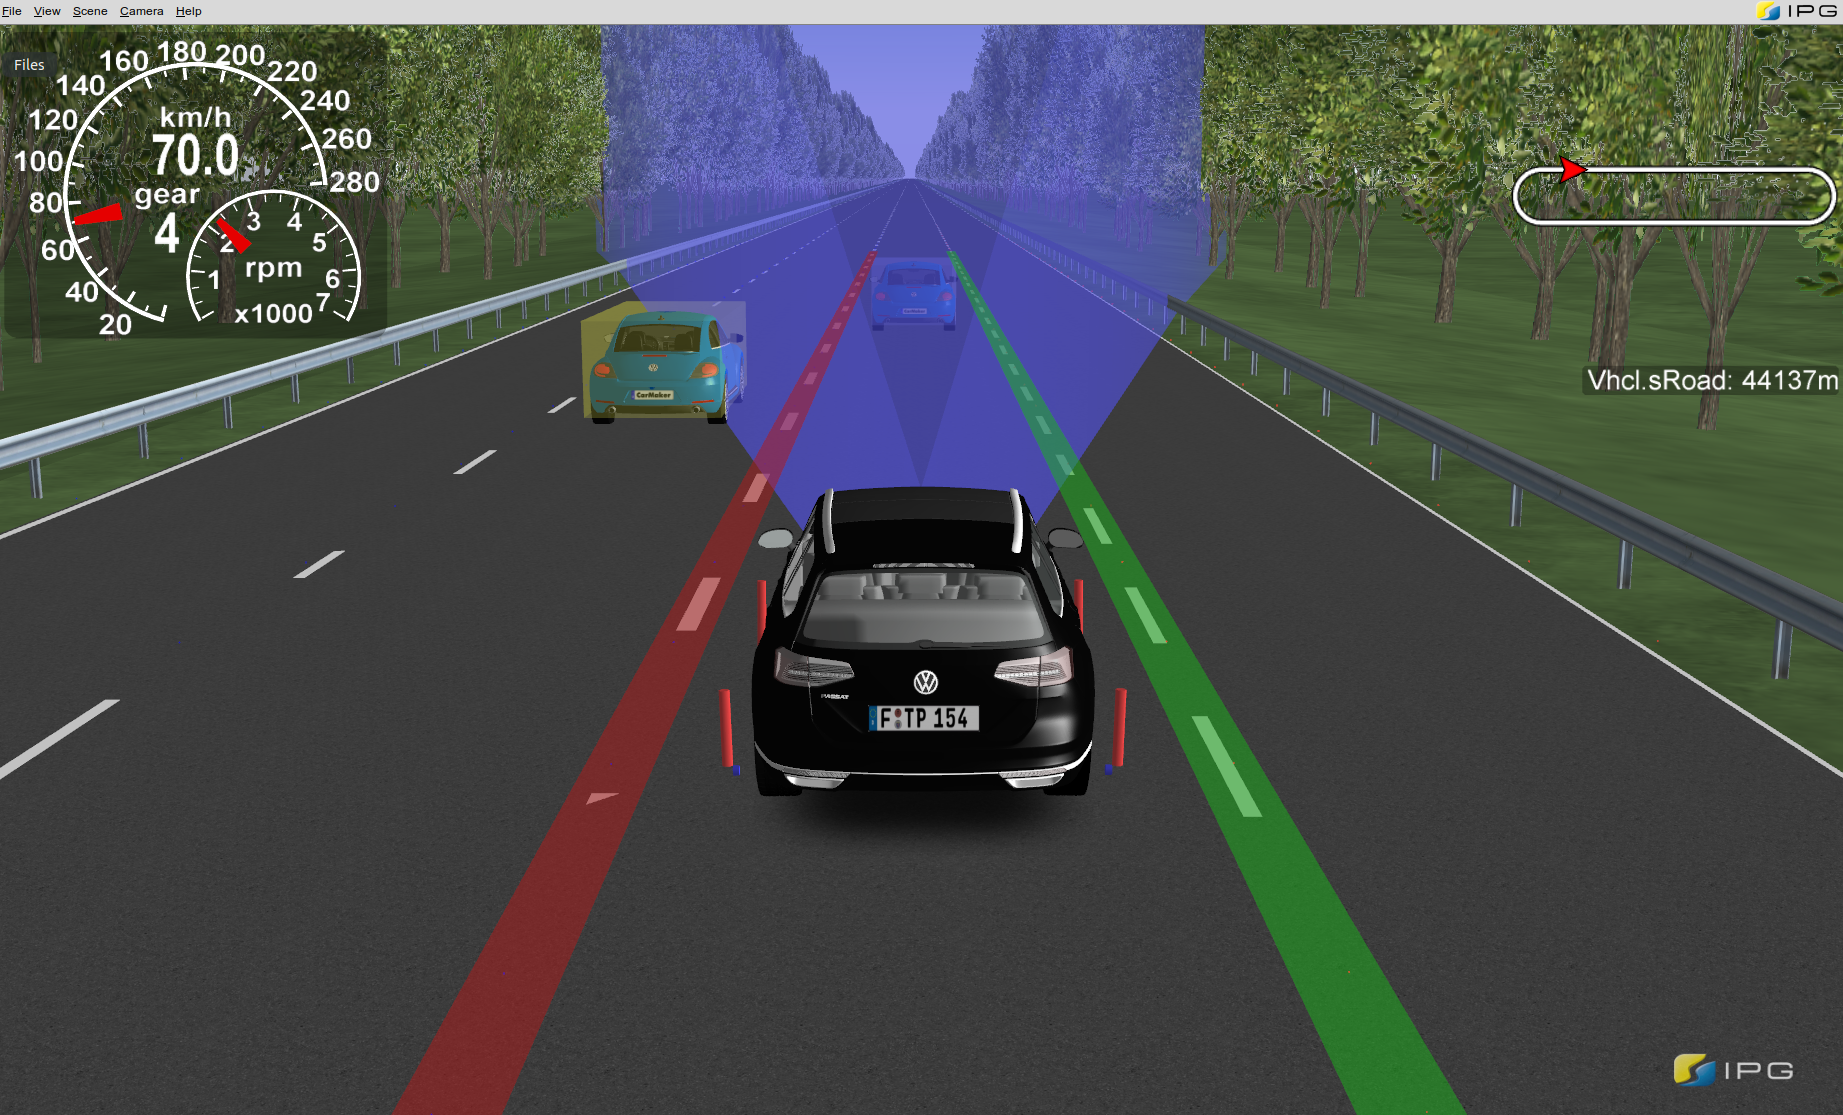
\includegraphics[width=1.0\linewidth]{Abbildungen/bericht/carmaker_lc_part1}
		\caption{Ausgangssituation: Ein TPO auf der Ego-Lane (rechts) sowie ein TPO auf der Target-Lane (links) }
		\label{fig.carmaker_lanechange_part1}
	\end{center}
\end{figure} 

\begin{figure}[!ht]
	\begin{center}
		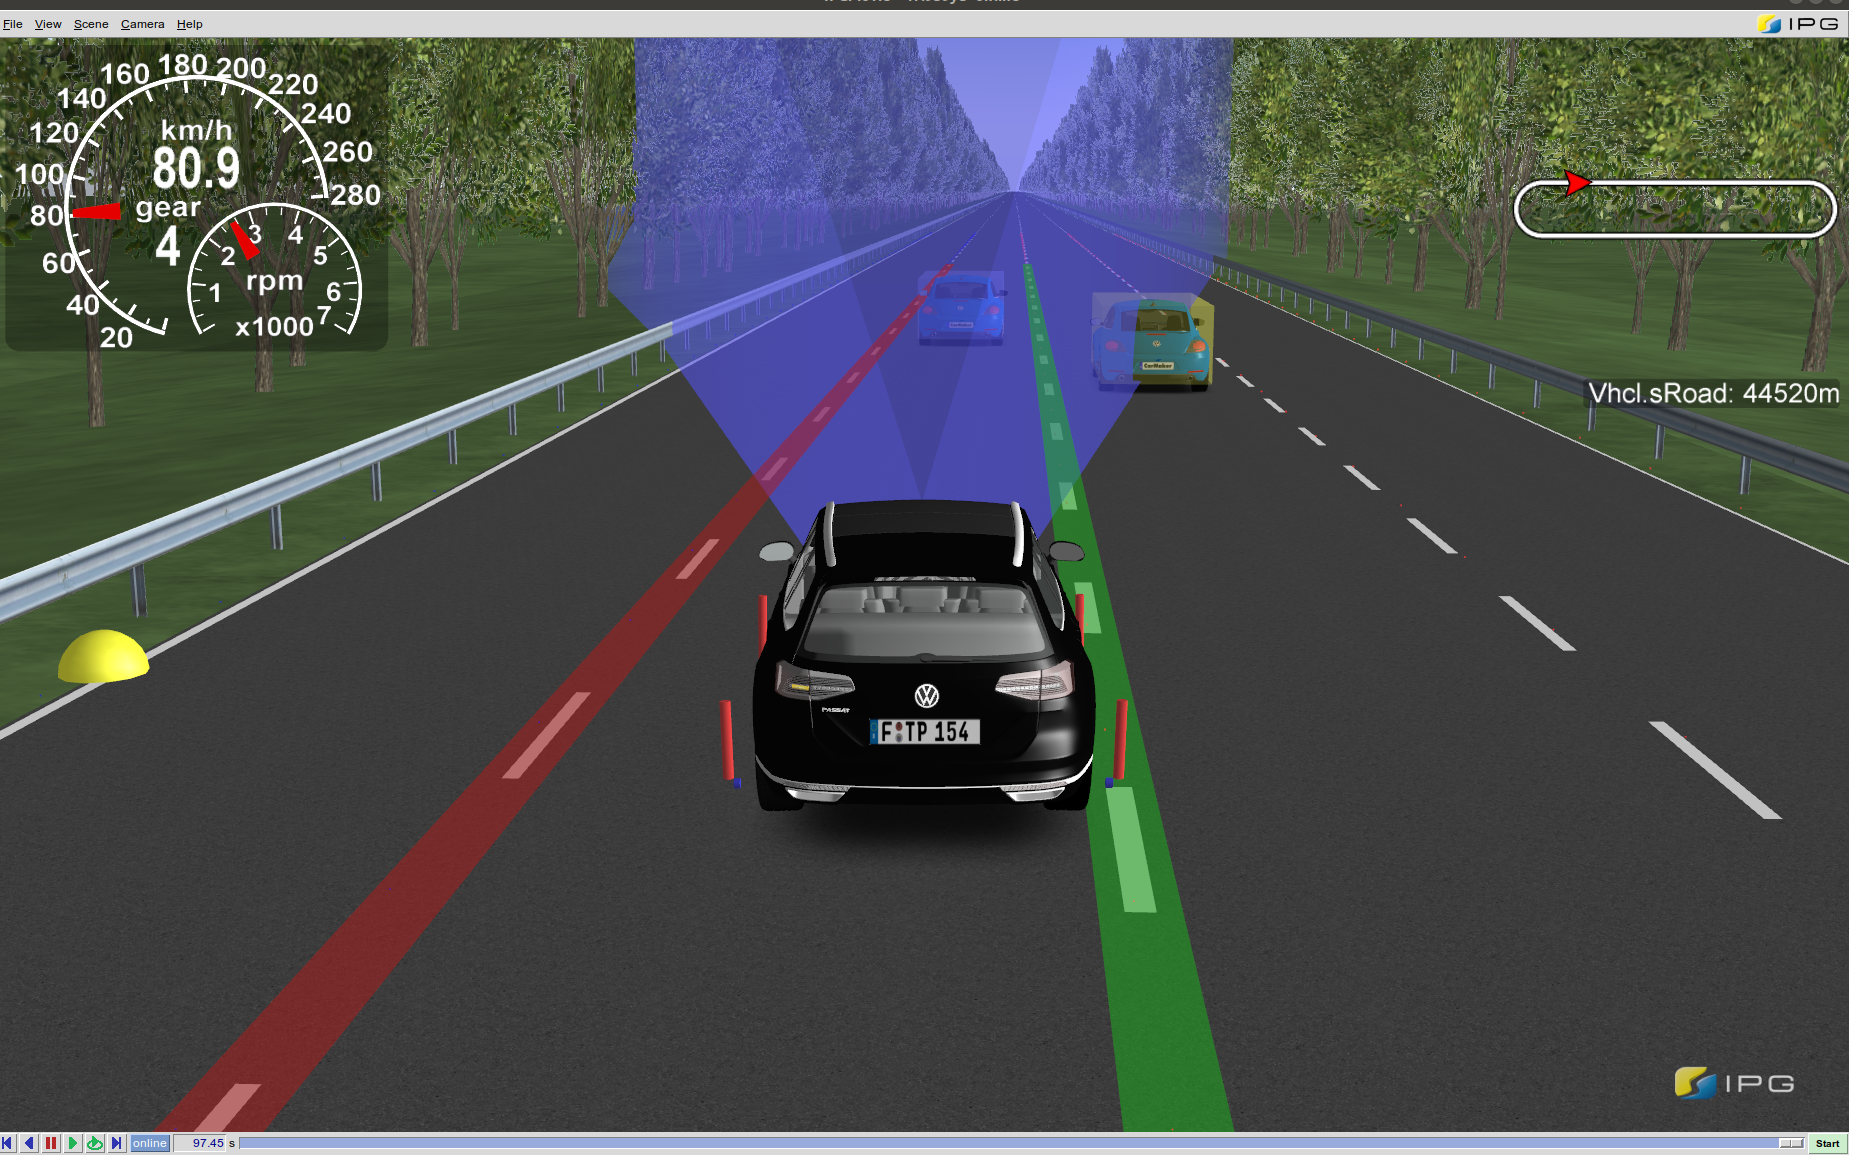
\includegraphics[width=1.0\linewidth]{Abbildungen/bericht/carmaker_lc_part2}
		\caption{Spurwechsel mit gleichförmig weiter fahrenden TPO's auf beiden Fahrspuren}
		\label{fig.carmaker_lanechange_part2}
	\end{center}
\end{figure} 

\begin{figure}[!ht]
	\begin{center}
		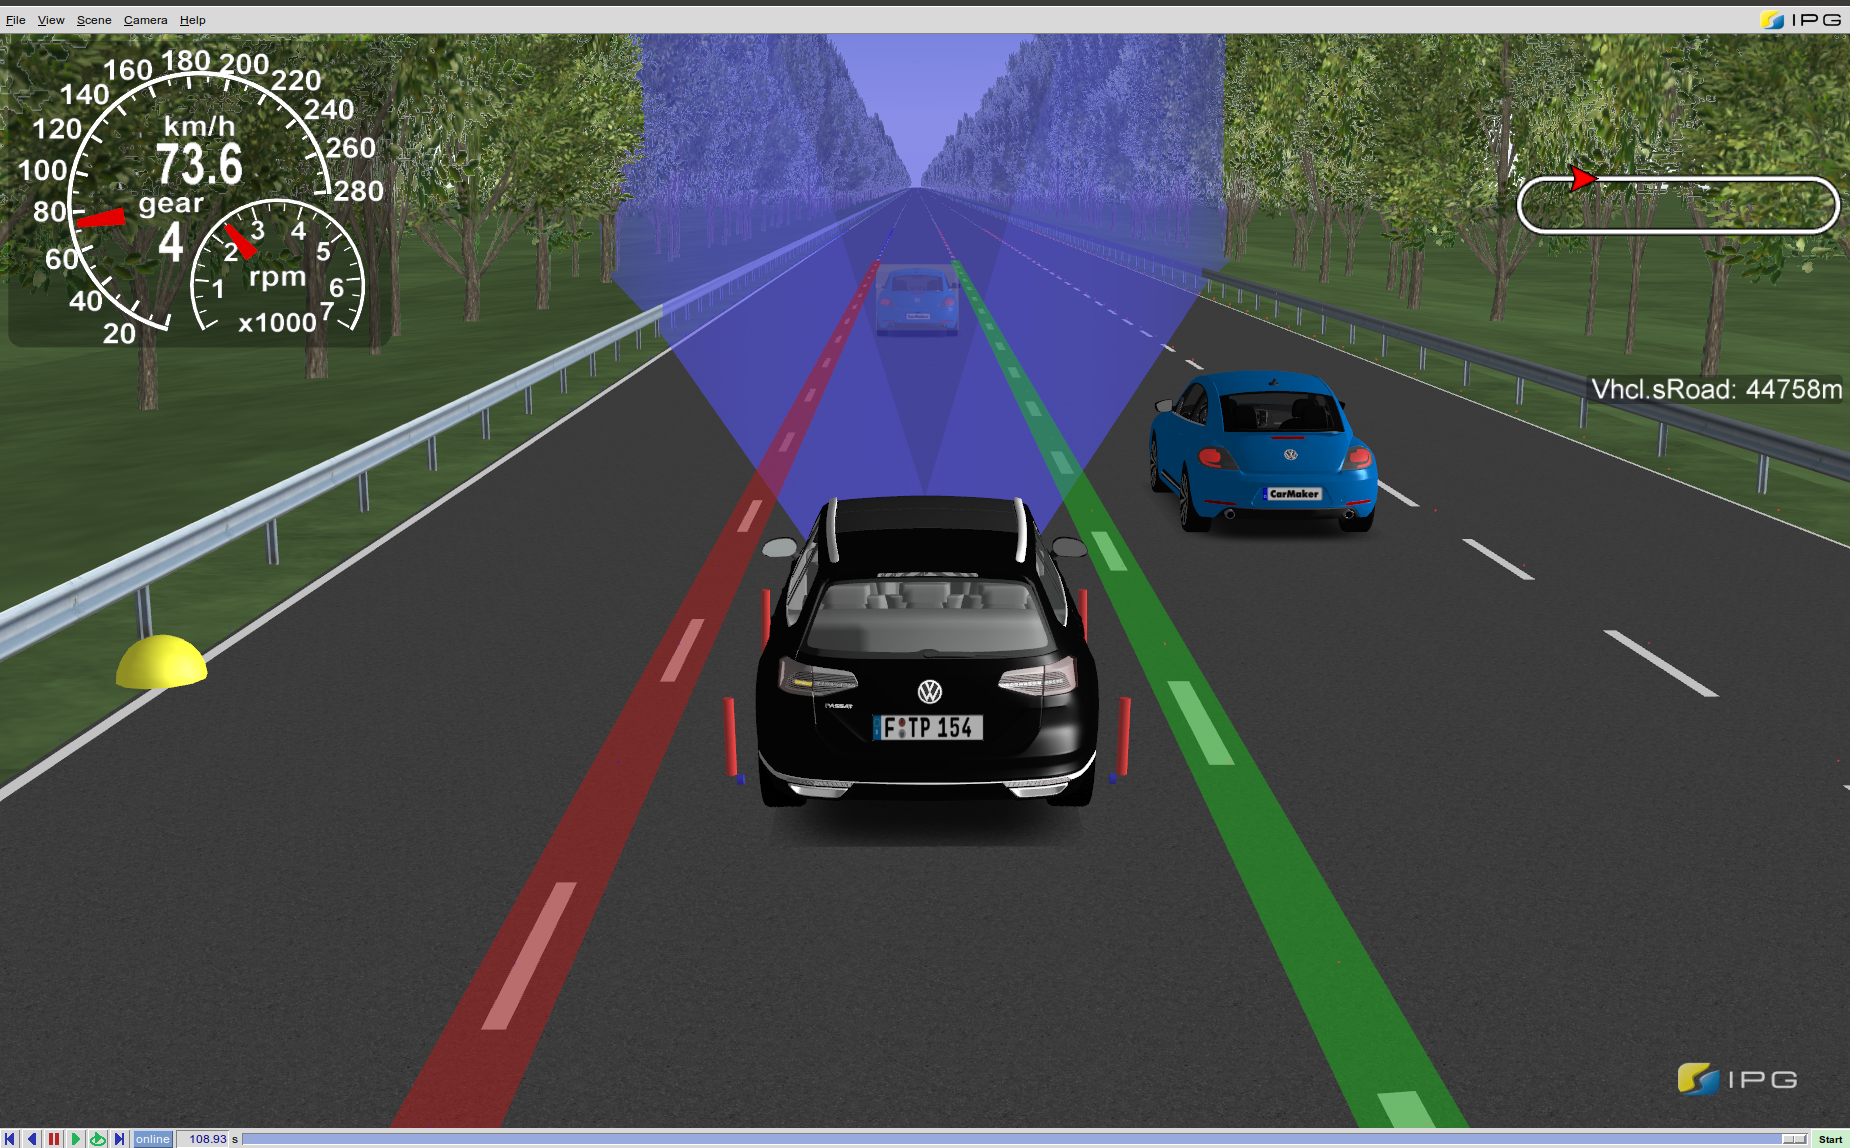
\includegraphics[width=1.0\linewidth]{Abbildungen/bericht/carmaker_lc_part3}
		\caption{Manöverende: Ego-Fahrzeug befindet sich auf der Target-Lane und setzt Fahrt fort}
		\label{fig.carmaker_lanechange_part3}
	\end{center}
\end{figure} 

In Bild xx sind neben dem Ego-Fahrzeug (schwarzer VW Passat) und den beiden TPO's (blaue VW Beetles) in der rechten, oberen Ecke die aktuelle Geschwindigkeit sowie die Radumdrehungen pro Minute eingezeichnet. In der rechten oberen Ecke findet sich die Übersicht der Teststrecke, auf denen sich die Fahrzeuge befinden. Der blaue Lichtkegel, welcher in dem Bild zu sehen ist, repräsentiert den Detektionsbereich des Radars, mit dem das Ego-Fahrzeug ausgestattet ist. Durch die vorverarbeiteten Umweltinformationen (siehe Abbildung xx Systemarchitektur) konnten die beiden TPO's detektiert werden und sind von gelben Detektionskästen umgeben. Die Lane-Marker der aktuellen Ego-Lane sind in grün (rechte Fahrspur-Begrenzung) sowie rot (linke Fahrspur-Begrenzung) eingezeichnet. Während des Spurwechsels wird wechseln die ausgewählten Lane-Marker nun (siehe Bild xx), da sich zeitgleich die aktuelle Spur des Ego-Fahrzeuges geändert hat. Nach dem erfolgreichen Spurwechsel wird die Fahrt nun unter Berücksichtigung der Sollgeschwindigkeit, aber primär unter Einhaltung des Sicherheitsabstandes zum vor dem Ego-Fahrzeug fahrenden TPO (siehe Bild xxx), gleichförmig fortgesetzt.

Als Ergebnis der drei Testszenarien standen Messdaten, welche mit Hilfe eines Analyse-Tools weiteren Untersuchungen unterzogen werden mussten. Die Daten ermöglichen ein \glqq Wiederabspielen\grqq{} der Simulationen. Hierzu betrachte man im Folgenden Bild xxx. 

\begin{figure}[!ht]
	\begin{center}
	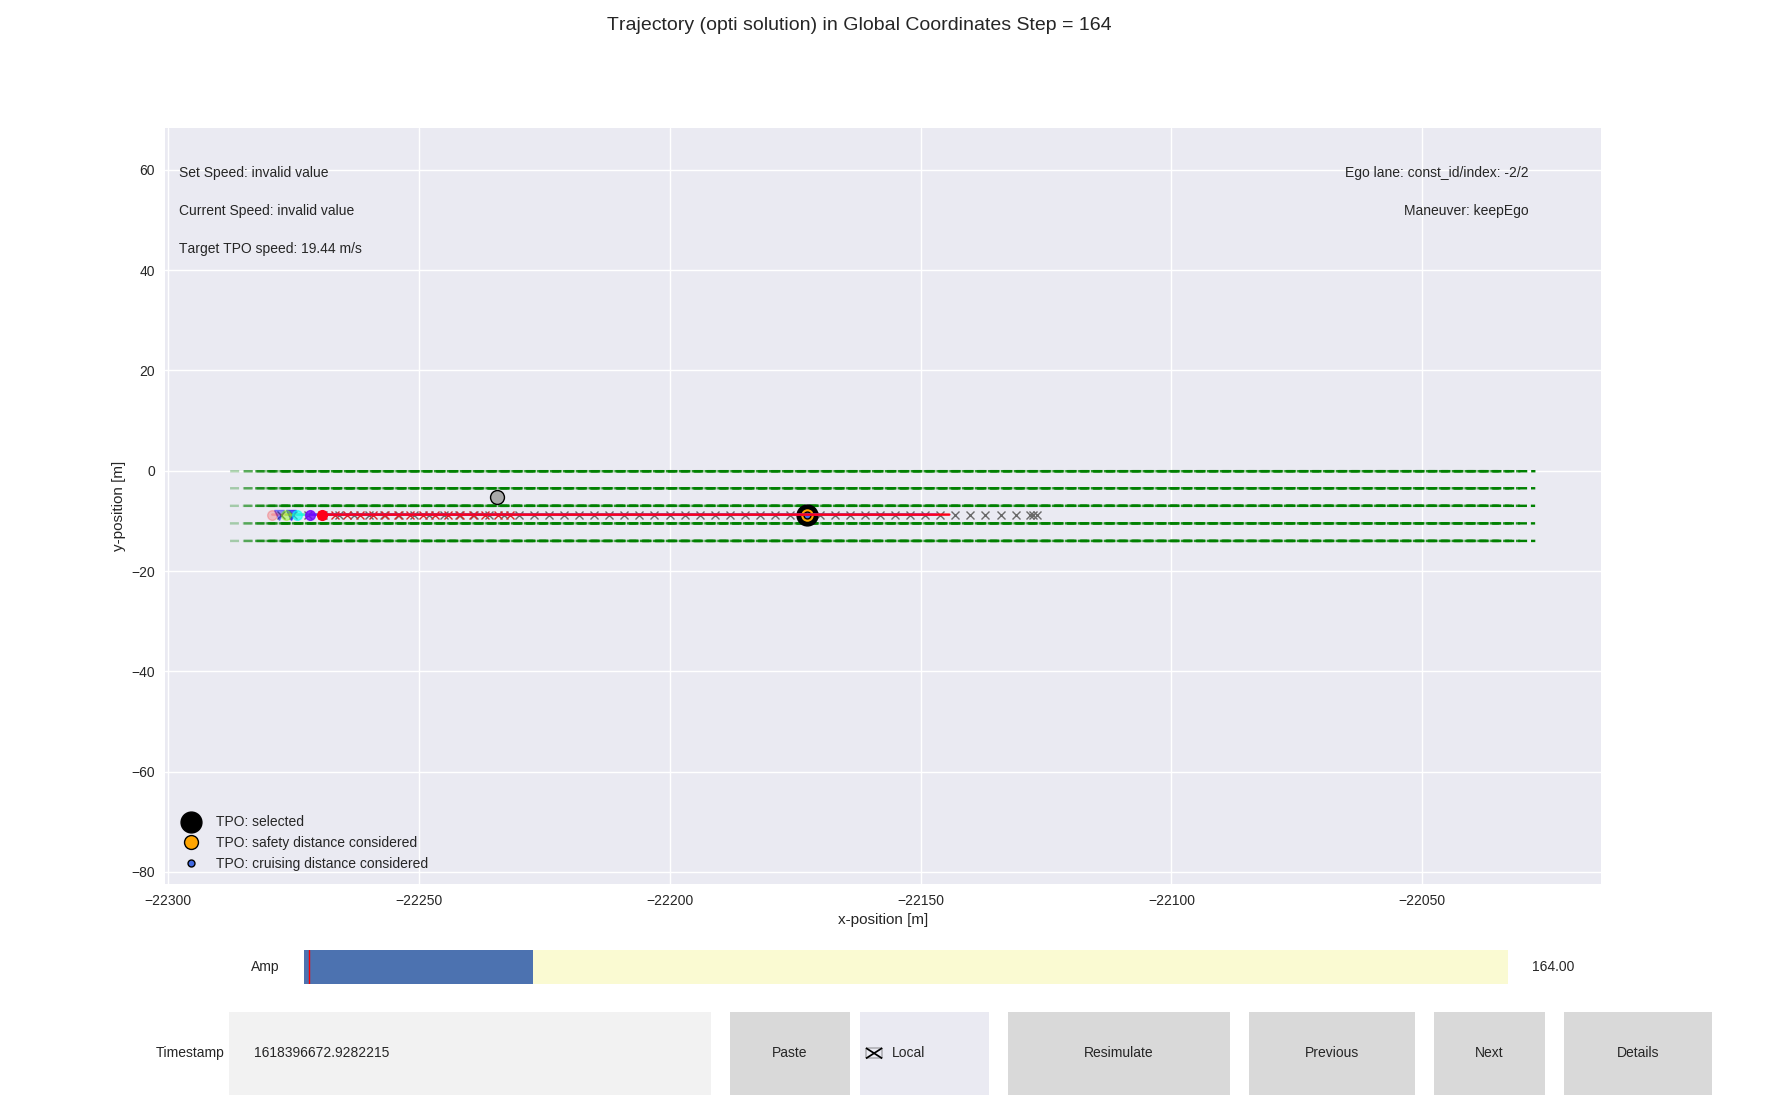
\includegraphics[width=1.0\linewidth]{Abbildungen/bericht/process_logged_data_lc_part1}
	\caption{Visualisierung der Verkehrssituation und der geplanten Fahrlinie}
	\label{fig.process_logged_data_part1}
\end{center}
\end{figure} 

Dieses spielt sich ca. zeitgleich zu der Szene in Bild xx ab. Die beiden Kreise repräsentieren die beiden TPO's. Da sich das Ego-Fahrzeug auf der rechten Spur befindet und noch kein Fahrspur-Wechsel durch Setzen des Blinkers angefragt wurde, ist das vor dem Ego-Fahrzeug fahrende TPO das für das ACC entscheidende Fahrzeug. Dieses TPO bestimmt die \glqq cruising distance\grqq{} wie auch die \glqq safety distance\grqq{}, welches ein noch einmal verschärfter Sicherheitsbereich, der nicht von dem Ego-Fahrzeug verletzt werden darf, repräsentiert. Die \grqq safety distance\grqq{} ist hierbei die in Bild xx grau schraffierte Fläche. Die \glqq Solltrajektorie\grqq{}, also die gewünschte Abfolge von Fahrpositionen des Ego-Fahrzeuges, ist in dem Bild xx anhand der grauen \glqq x\grqq{}-Markierungen dargestellt. Dies kann dadurch begründet werden, dass zu dem Zeitpunkt noch kein Blinker als Signal eines Spurwechsels gesetzt wurde, und die aktuelle Wunschtrajektorie schlicht der aktuellen Fahrbahn folgt. Die von den Algorithmen geplante Trajektorie für die unmittelbare Zukunft ist in Bild xx in rot dargestellt. Es ist zu erkennen, dass die geplante Trajektorie die gewünschte Trajektorie sehr genau abbildet.

\begin{figure}[!ht]
	\begin{center}
		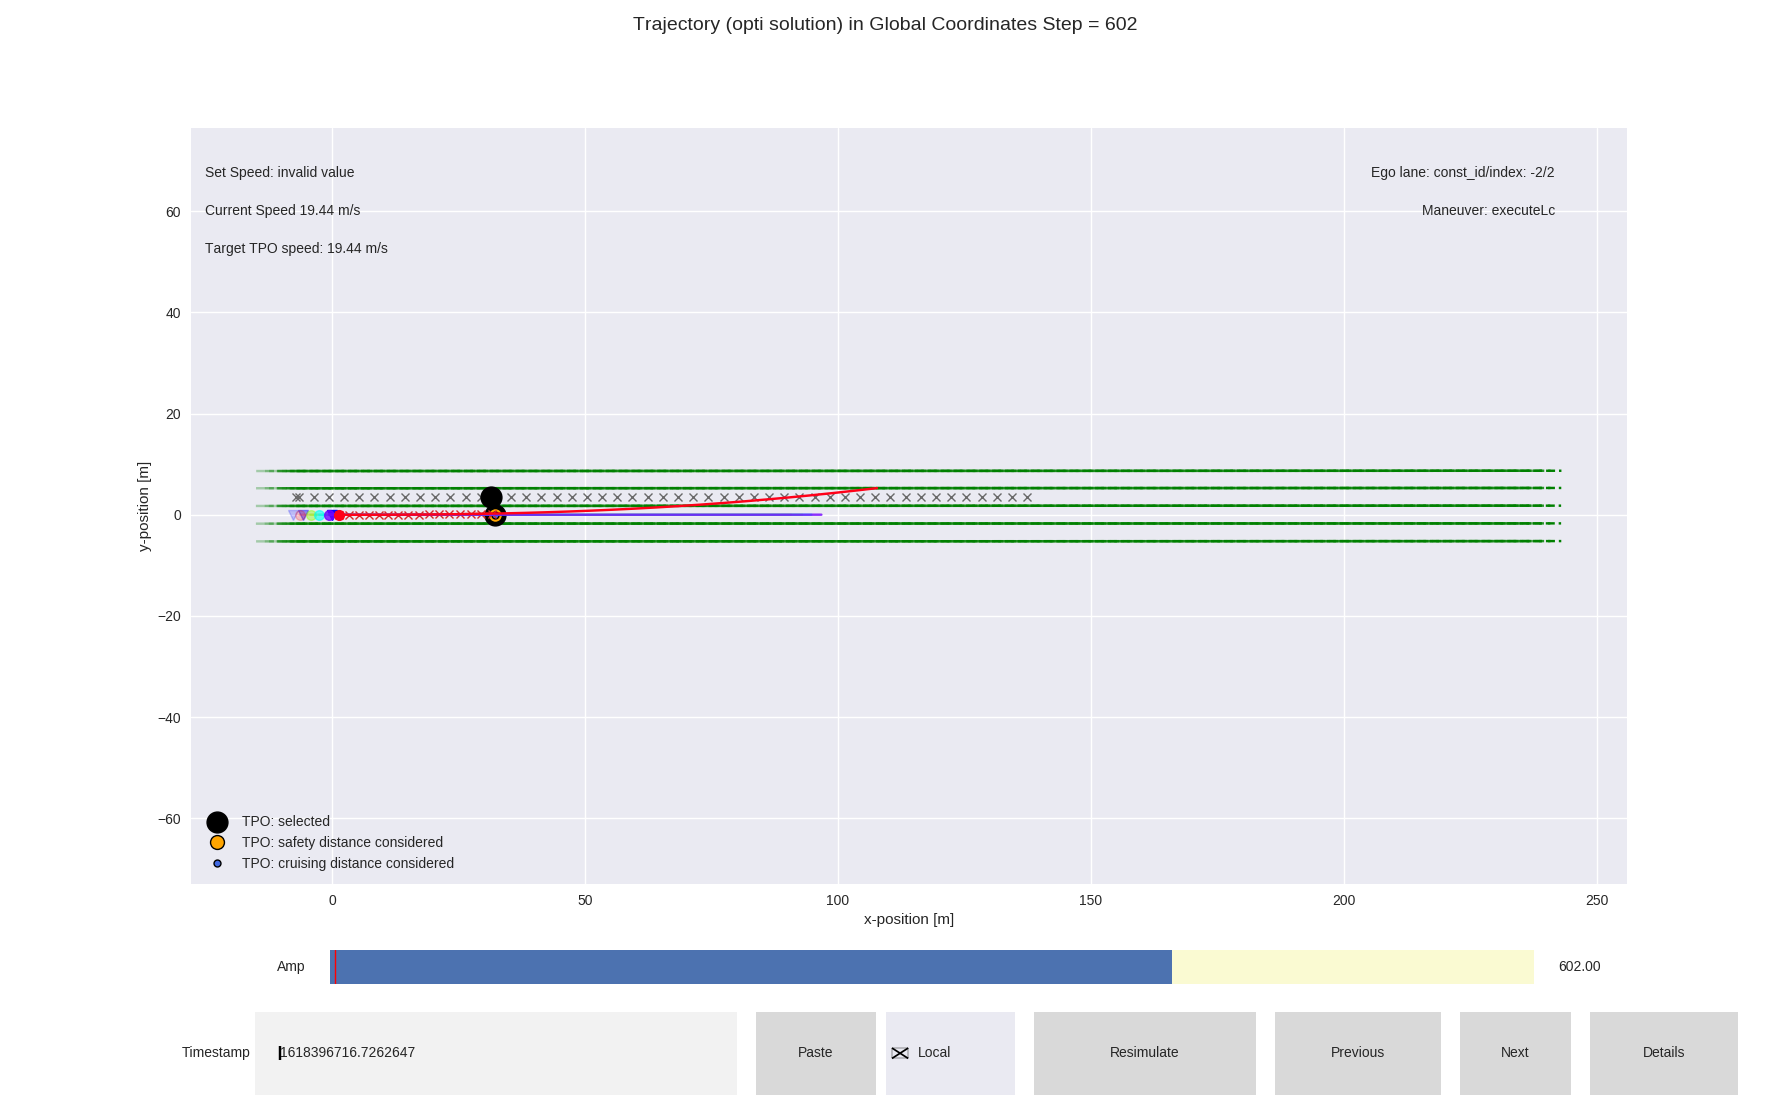
\includegraphics[width=1.0\linewidth]{Abbildungen/bericht/process_logged_data_lc_part2}
		\caption{M}
		\label{fig.process_logged_data_part2}
	\end{center}
\end{figure}  

Die Auswirkungen des Setzens des Blinkers werden nun in Abbildung xx deutlich. So sendet das Setzen des Blinkers an den Trajektorienplaner das Signal, dass die neue Target-Lane die links neben dem Ego-Fahrzeug befindliche Spur ist. Dementsprechend liegt in Bild xx die durch die grauen \glqq x'e\grqq{} gekennzeichnete Solltrajektorie auf der linken Spur. Mittels mehrerer Iterationen versucht der Trajektorienplaner, eine optimale Trajektorie zu finden. Liegt diese in einem ersten Schritt noch auf der aktuellen Ego-Fahrbahn (blaue Trajektorie in Bild xx), so führt sie schon nach einer weiteren Iteration auf die gewünschte Sollfahrbahn (rote Trajektorie in Bild xx). Da zu diesem Zeitpunkt weiterhin das vor dem Ego-Fahrzeug befindliche TPO für die \glqq Adaptive Cruise Control\grqq{} maßgeblich ist, sind weiterhin dessen \glqq safety distance\grqq{} sowie \glqq cruising distance\grqq{} vom Trajektorienplaner ausgewählt (man beachte die blaue und gelbe Markierung, welche auf dem Ego-Lane TPO liegen).
